\clearpage
\VerdierPhysicalPageAnchor{0140}%
\begingroup
\normalsize
\setlength{\parskip}{0pt}%
\setlength{\emergencystretch}{1.5em}%
\setlength{\abovedisplayskip}{1pt plus 1pt minus 1pt}%
\setlength{\belowdisplayskip}{1pt plus 1pt minus 1pt}%

\VerdierSemanticAnchor{ch2-2-2-6-proof-b-triii-completion}
\noindent 则存在态射 $r\colon Q(Z)\longrightarrow Q(Z')$，使
$(m,p,r)$ 为三角的态射。
\VerdierSemanticAnchor{ch2-2-2-6-proof-b-triii-case-reduction}%
利用引理 (2.2.7)，问题归结为考察下列两种情形：

\VerdierSemanticAnchor{ch2-2-2-6-proof-b-triii-case-a}
\noindent\textit{a)}\quad
$m=Q(s)^{-1}$，$p=Q(t)^{-1}$，$s,t\in S$，且图式：

\VerdierSemanticAnchor{ch2-2-2-6-proof-b-triii-case-a-square}
\begin{center}
  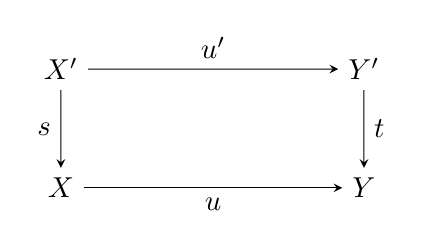
\begin{tikzpicture}[>=stealth,line width=.38pt,x=1.85cm,y=1.45cm,
    scale=1.04,transform shape]
    \node (Xp) at (0,1) {$X'$};
    \node (Yp) at (2,1) {$Y'$};
    \node (X)  at (0,0) {$X$};
    \node (Y)  at (2,0) {$Y$};
    \draw[->] (Xp) -- node[above] {$u'$} (Yp);
    \draw[->] (Xp) -- node[left] {$s$} (X);
    \draw[->] (Yp) -- node[right] {$t$} (Y);
    \draw[->] (X) -- node[below] {$u$} (Y);
  \end{tikzpicture}
\end{center}

\noindent 交换。

\VerdierSemanticAnchor{ch2-2-2-6-proof-b-triii-case-b}
\noindent\textit{b)}\quad
$m=Q(f)$，$p=Q(g)$，且图式：

\VerdierSemanticAnchor{ch2-2-2-6-proof-b-triii-case-b-square}
\begin{center}
  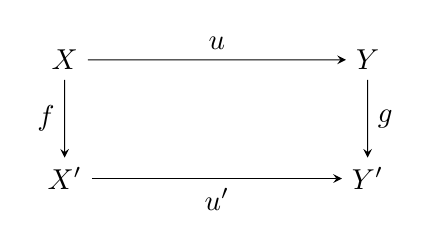
\begin{tikzpicture}[>=stealth,line width=.38pt,x=1.85cm,y=1.45cm,
    scale=1.04,transform shape]
    \node (X)  at (0,1) {$X$};
    \node (Y)  at (2,1) {$Y$};
    \node (Xp) at (0,0) {$X'$};
    \node (Yp) at (2,0) {$Y'$};
    \draw[->] (X) -- node[above] {$u$} (Y);
    \draw[->] (X) -- node[left] {$f$} (Xp);
    \draw[->] (Y) -- node[right] {$g$} (Yp);
    \draw[->] (Xp) -- node[below] {$u'$} (Yp);
  \end{tikzpicture}
\end{center}

\noindent 交换。

\VerdierSemanticAnchor{ch2-2-2-6-proof-b-triii-case-conclusion}
\noindent 在情形 \textit{a)} 中，所需性质由性质 SM6) (2.1.2) 得到。
在情形 \textit{b)} 中，所需性质由 $\mathcal D$ 的特异三角的性质
TRIII 得到。

\VerdierSemanticAnchor{ch2-2-2-8}
\smallskip
\noindent\textbf{2.2.8.\quad 引理 2.2.7 的证明。}
\VerdierSemanticAnchor{ch2-2-2-8-initial-lift}%
由定理 (2.2.2)，存在态射 $t\colon Y''\longrightarrow Y$，$t\in S$，
使 $pQ(t)=Q(g)$，其中 $g\colon Y''\longrightarrow Y'$。然后逐步构造
下列图式：

\VerdierSemanticAnchor{ch2-2-2-8-stepwise-diagram}
\begin{center}
  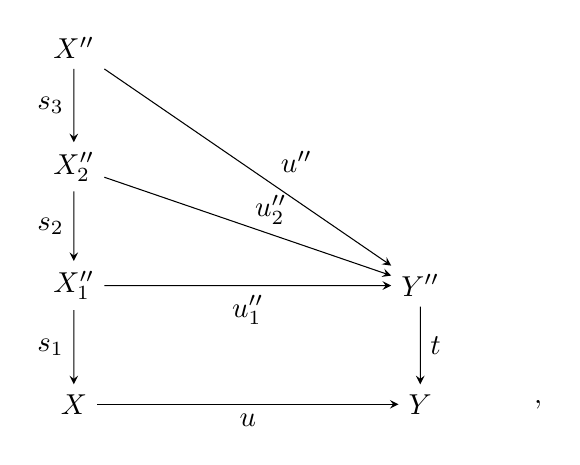
\begin{tikzpicture}[>=stealth,line width=.38pt,x=1.80cm,y=1.45cm,
    scale=1.04,transform shape]
    \node (Xpp)  at (0,3) {$X''$};
    \node (X2pp) at (0,2) {$X_2''$};
    \node (X1pp) at (0,1) {$X_1''$};
    \node (X)    at (0,0) {$X$};
    \node (Ypp)  at (2.35,1) {$Y''$};
    \node (Y)    at (2.35,0) {$Y$};
    \draw[->] (Xpp) -- node[left] {$s_3$} (X2pp);
    \draw[->] (X2pp) -- node[left] {$s_2$} (X1pp);
    \draw[->] (X1pp) -- node[left] {$s_1$} (X);
    \draw[->] (Xpp) -- node[pos=.58,above right] {$u''$} (Ypp);
    \draw[->] (X2pp) -- node[pos=.58,above] {$u_2''$} (Ypp);
    \draw[->] (X1pp) -- node[below] {$u_1''$} (Ypp);
    \draw[->] (Ypp) -- node[right] {$t$} (Y);
    \draw[->] (X) -- node[below] {$u$} (Y);
    \node at (3.15,0) {$,$};
  \end{tikzpicture}
\end{center}

\VerdierSemanticAnchor{ch2-2-2-8-proof-p141-boundary}
\VerdierSemanticAnchor{ch2-2-2-8-p141-boundary}
\endgroup
